\documentclass[18pt,xcolor=table]{beamer}
% -----PACKAGES
%\usepackage[shortend,titlenumbered]{algorithm2e}
%\usepackage{algorithmic}
%\usepackage[plain]{algorithm}
\usepackage{multicol}
\usepackage{color}
\usepackage{multirow}
\usepackage{fancybox}
%\usepackage{index}
\usepackage{varioref}
\usepackage{psfrag}
\usepackage{epsfig}
\usepackage{boxedminipage}
\usepackage{graphicx}
\usepackage{rotating}
\usepackage{amsmath}
\usepackage{amssymb}
%\usepackage{amsfont}
\usepackage{latexsym}
\usepackage{alltt}
%\usepackage[small,bf]{caption}
\usepackage{url}
%\usepackage{citesort}
%\usepackage{crop}
\usepackage{array}
\usepackage{subfigure}
\usepackage{dcolumn}

% -----SETLENGTH
%\setlength{\captionmargin}{20pt} 

% -----NEWCOMMANDS
\newcommand{\nc}{\newcommand}
\nc{\mathsm}[1]{\text{\small{$#1$}}}
\nc{\ubar}[1]{\underset{-}{#1}}
\nc{\optype}{\textrm}
\nc{\EQ}[1]{(\ref{eq:#1})}
\nc{\TAB}[1]{\ref{tab:#1}}
\nc{\FIG}[1]{\ref{fig:#1}}
\nc{\SEC}[1]{\ref{sec:#1}}
\nc{\ALG}[1]{\ref{alg:#1}}
\nc{\CHAP}[1]{\ref{chap:#1}}
\nc{\mtrx}[1]{\boldsymbol{\mathbf{#1}}}
\nc{\vctr}[1]{\boldsymbol{\mathbf{#1}}}
\nc{\grad}{\mbox{\boldmath$\nabla$}}
\nc{\gradient}{\textsl{grad}\,}
\nc{\hessian}{\textsl{grad\,}^2}
\nc{\ii}{\iota}
\nc{\dd}{d}
\nc{\ee}{\mathrm{e}}
\nc{\pdiv}[2]{\partial{#1}/\partial{#2}}
\nc{\dpdiv}[2]{\displaystyle{\frac{\partial{#1}}{\partial{#2}}}}
\nc{\ddiv}[2]{\displaystyle{\frac{\dd{#1}}{\dd{#2}}}}
\nc{\inpr}{\hspace{-1pt}\cdot\hspace{-1pt}}
\nc{\IR}{\mathbb{R}}
\nc{\IN}{\mathbb{N}}
\nc{\IZ}{\mathbb{Z}}
\nc{\IC}{\mathbb{C}}
\nc{\half}{\frac{1}{2}}
\nc{\shalf}{\scriptstyle{\half}} 
\nc{\ds}[1]{\displaystyle{#1}}
\nc{\ts}[1]{\textstyle{#1}}
\nc{\sign}{\optype{sign}}
\nc{\spr}{\optype{spr}}
\nc{\dist}{\optype{dist}}
\nc{\rank}{\optype{rank}}
\nc{\codim}{\optype{codim}}
\nc{\supp}{\optype{supp}}
\nc{\diag}{\optype{diag}}
\nc{\meas}{\optype{meas}}
\nc{\cond}{\optype{cond}}
\nc{\kernel}{\optype{kernel}}
\nc{\spa}{\optype{span}}
\nc{\order}{\mathcal{O}}
\nc{\Fr}{\mathrm{Fr}}
\nc{\Rey}{\mathrm{Re}}
\nc{\Ord}{O}
\nc{\ord}{o}
\nc{\st}{\:{:}\:}
\nc{\closure}[1]{\overline{#1}}
\nc{\emin}[1]{\emph{#1}\index{#1}\/}
\nc{\rmin}[1]{#1\index{{}@{#1}}}
\nc{\Laplace}{\Delta}
\nc{\ie}{i.e.}
\nc{\eg}{e.g.}
%\nc{\union}{\cup}
\nc{\Union}{\bigcup}
\nc{\lf}[1]{\mathsf{#1}}
\nc{\dbar}[1]{\bar{\bar{#1}}}
\nc{\ul}[1]{\underline{#1}}
\nc{\hpt}{\hspace{0.5pt}}
\nc{\E}[1]{\times{}10^{#1}}
\nc{\inp}[2]{\langle{#1},{#2}\rangle}
\nc{\tmpcommand}{}

% -----RENEWCOMMANDS
\renewcommand{\baselinestretch}{1}
\renewcommand{\exp}{\optype{exp}\,}
\renewcommand{\cosh}{\optype{cosh}\,}
\renewcommand{\tanh}{\optype{tanh}\,}
\renewcommand{\sinh}{\optype{sinh}\,}
\renewcommand{\div}[1]{\optype{div}\,{#1}}
\renewcommand{\half}{\mbox{$\frac{1}{2}$}}
%\renewcommand{\descriptionlabel}[1]{\hspace{\labelsep}\emph{#1}}

% -----ETC
\raggedbottom


\DeclareMathOperator{\curl}{\bf curl}
\DeclareMathOperator{\rot}{\rm curl}
\DeclareMathOperator{\divv}{\rm div}
\newcommand{\tro}{\gamma_0}
\newcommand{\trt}{\gamma_{\sft}}
\newcommand{\trn}{\gamma_{\sfn}}

\newcommand{\PT}{{\partial T}}
\newcommand{\bbN}{{\mathbb{N}}}
\newcommand{\bbP}{{\mathbb{P}}}

\newcommand{\scC}{{\mathscr{C}}}
\newcommand{\caD}{{\mathcal{D}}}
\newcommand{\caL}{{\mathcal{L}}}

\newcommand{\sfe}{{\mathsf{e}}}
\newcommand{\sff}{{\mathsf{f}}}
\newcommand{\sft}{{\boldsymbol{\mathsf{t}}}}
\newcommand{\sfn}{{\boldsymbol{\mathsf{n}}}}

%   Common caligraphic abbrevs
\newcommand{\BB}{\mathcal{B}}
\newcommand{\CC}{\mathcal{C}}
\newcommand{\DD}{\mathcal{D}}
\newcommand{\EE}{\mathcal{E}}
\newcommand{\FF}{\mathcal{F}}
\newcommand{\GG}{\mathcal{G}}
\newcommand{\II}{\mathcal{I}}
\newcommand{\JJ}{\mathcal{J}}
\newcommand{\KK}{\mathcal{K}}
\newcommand{\LL}{\mathcal{L}}
\newcommand{\OO}{\mathcal{O}}
\newcommand{\QQ}{\mathcal{Q}}
\newcommand{\RR}{\mathcal{R}}
\newcommand{\TT}{\mathcal{T}}


 %% JAY'S PREAMBLE
 %%========================

%   Math symbol definitions
\def\d{\partial}
%\newsymbol\lee 132E
\newcommand{\union}{\mathop{\bigcup}}
\newcommand{\intersect}{\mathop{\bigcap}}
\newcommand{\binomial}[2]{\ensuremath{
		\begin{pmatrix}{#1}\\{#2}\end{pmatrix}}}
\newcommand{\smallbinomial}[2]{\ensuremath{
		(\begin{smallmatrix}{#1}\\{#2}\end{smallmatrix})}}
\newcommand{\tang}[1]{\ensuremath{{#1}_{\intercal}}} % can use \top
						     % also
\newcommand{\hypergeom}[2]{\ensuremath{\sideset{_{#1}}{_{#2}}{\mathop{F}}}}
%   Difficult names
\newcommand{\Babuska}{Babu{\v{s}}ka}       % Remember: Usage is \Babuska\
\newcommand{\Cea}{C{\'e}a}                 % with trailing `\' to give space
\newcommand{\Poincare}{Poincar{\'{e}}}     % when needed, but when ending
\newcommand{\Nedelec}{N{\'{e}}d{\'{e}}lec} % sentence use \Babuska.
\newcommand{\Frechet}{Fr{\'{e}}chet}
\newcommand{\Muller}{M{\"u}ller}
\newcommand{\LHospital}{L'H{\^{o}}spital}
%   Bold and beautiful
\newcommand{\ba}{{\boldsymbol{a}}}
\newcommand{\bA}{\boldsymbol{A}}
\newcommand{\balpha}{{\boldsymbol{\alpha}}}
\newcommand{\bB}{{\boldsymbol{B}}}
\newcommand{\bb}{{\boldsymbol{b}}}
\newcommand{\bbeta}{{\boldsymbol{\beta}}}
\newcommand{\etab}{{\boldsymbol{\eta}}}
\newcommand{\bC}{{\boldsymbol{C}}}
\newcommand{\bc}{{\boldsymbol{c}}}
\newcommand{\bD}{{\boldsymbol{D}}}
\newcommand{\bd}{{\boldsymbol{d}}}
\newcommand{\db}{{\boldsymbol{\d}}}
\newcommand{\bdelta}{{\boldsymbol{\delta}}}
\newcommand{\bDelta}{{\boldsymbol{\Delta}}}
\newcommand{\beps}{{\boldsymbol{\varepsilon}}}
\newcommand{\be}{{\boldsymbol{e}}}
\newcommand{\bg}{{\boldsymbol{g}}}
\newcommand{\bm}{{\boldsymbol{m}}}
\newcommand{\bn}{{\boldsymbol{n}}}
\newcommand{\bN}{{\boldsymbol{N}}}
\newcommand{\bp}{{\boldsymbol{p}}}
\newcommand{\bpsi}{{\boldsymbol{\psi}}}
\newcommand{\bq}{{\boldsymbol{q}}}
\newcommand{\bxi}{{\boldsymbol{\xi}}}
\newcommand{\bE}{{\boldsymbol{E}}}
\newcommand{\bF}{{\boldsymbol{F}}}
\newcommand{\bh}{{\boldsymbol{h}}}
\newcommand{\bH}{{\boldsymbol{H}}}
\newcommand{\bI}{{\boldsymbol{I}}}
\newcommand{\bj}{{\boldsymbol{j}}}
\newcommand{\bJ}{{\boldsymbol{J}}}
\newcommand{\bK}{{\boldsymbol{K}}}
\newcommand{\bk}{{\boldsymbol{k}}}
\newcommand{\bll}{{\boldsymbol{\ell}}}
\newcommand{\bL}{{\boldsymbol{L}}}
\newcommand{\blambda}{{\boldsymbol{\lambda}}}
\newcommand{\bmu}{{\boldsymbol{\mu}}}
\newcommand{\bM}{{\boldsymbol{M}}}
\newcommand{\bomega}{{\boldsymbol{\omega}}}
\newcommand{\bP}{{\boldsymbol{P}}}
\newcommand{\bphi}{{\boldsymbol{\phi}}}
\newcommand{\bQ}{{\boldsymbol{Q}}}
\newcommand{\bG}{{\boldsymbol{G}}}
\newcommand{\bu}{{\boldsymbol{u}}}
\newcommand{\bU}{{\boldsymbol{U}}}
\newcommand{\bV}{{\boldsymbol{V}}}
\newcommand{\bX}{{\boldsymbol{X}}}
\newcommand{\bv}{{\boldsymbol{v}}}
\newcommand{\bw}{{\boldsymbol{w}}}
\newcommand{\bW}{{\boldsymbol{W}}}
\newcommand{\bR}{{\boldsymbol{R}}}
\newcommand{\br}{{\boldsymbol{r}}}
\newcommand{\bS}{{\boldsymbol{S}}}
\newcommand{\bT}{{\boldsymbol{T}}}
\newcommand{\btau}{{\boldsymbol{\tau}}}
\newcommand{\bt}{{\boldsymbol{t}}}
\newcommand{\bx}{{\boldsymbol{x}}}
\newcommand{\by}{{\boldsymbol{y}}}
\newcommand{\bz}{{\boldsymbol{z}}}
\newcommand{\bzero}{{\boldsymbol{0}}}
\newcommand{\bZ}{{\boldsymbol{Z}}}
%   Common scalar fields
\newcommand{\RRR}{\mathbb{R}}
\newcommand{\CCC}{\mathbb{C}}
\newcommand{\ZZZ}{\mathbb{Z}}
\newcommand{\NNN}{\mathbb{N}}
%   Differential operators
\newcommand{\dive}{\mathop\mathrm{div}}
%\newcommand{\grad}{\ensuremath{\mathop{{\bf{grad}}}}}
%\newcommand{\curl}{{\ensuremath\mathop{\mathbf{curl}\,}}}
\newcommand{\Curl}{ {\bf Curl}}
\newcommand{\dx}{\ensuremath{\mathrm{d}x}}
\newcommand{\dy}{\ensuremath{\mathrm{d}y}}
\newcommand{\dr}{\ensuremath{\mathrm{d}r}}
\newcommand{\dR}{\ensuremath{\mathrm{d}R}}
\newcommand{\drho}{\ensuremath{\mathrm{d}\rho}}
\newcommand{\dz}{\ensuremath{\mathrm{d}z}}
\newcommand{\dzeta}{\ensuremath{\mathrm{d}\zeta}}
%   Wordy math symbols
\newcommand{\card}{\ensuremath{\mathop\mathrm{card}}}
%\newcommand{\diag}{\ensuremath{\mathop\mathrm{diag}}}
\newcommand{\diam}{\ensuremath{\mathop\mathrm{diam}}}
%\newcommand{\dist}{\mathop\mathrm{dist}}
\newcommand{\Ker}{\mathop\mathrm{Ker}}
\newcommand{\Range}{\mathop\mathrm{Range}}
%\newcommand{\rank}{\mathop\mathrm{rank}}
%\newcommand{\meas}{\mathop\mathrm{meas}}
\newcommand{\Forall}{\quad\text{for all }}
%\newcommand{\supp}{\mathop\mathrm{supp}}
\newcommand{\Span}{\mathop\mathrm{Span}}
\newcommand{\Hdiv}[1]{\bH(\dive,#1)}
%\newcommand{\Hcurl}[1]{\bH(\curl,#1)}
%   Common caligraphic abbrevs
%\newcommand{\BB}{\mathcal{B}}
%\newcommand{\CC}{\mathcal{C}}
%\newcommand{\DD}{\mathcal{D}}
%\newcommand{\EE}{\mathcal{E}}
%\newcommand{\FF}{\mathcal{F}}
%\newcommand{\GG}{\mathcal{G}}
%\newcommand{\II}{\mathcal{I}}
%\newcommand{\JJ}{\mathcal{J}}
%\newcommand{\KK}{\mathcal{K}}
%\newcommand{\LL}{\mathcal{L}}
%\newcommand{\OO}{\mathcal{O}}
%\newcommand{\QQ}{\mathcal{Q}}
%\newcommand{\RR}{\mathcal{R}}
%\newcommand{\TT}{\mathcal{T}}
%   Variations on standard symbols
\newcommand{\veps}{\varepsilon}
\newcommand{\vlam}{\varLambda}
\newcommand{\vpi}{\varPi}
\newcommand{\vPi}{\boldsymbol{\varPi}}
\newcommand{\vsig}{\varSigma}
\newcommand{\vbt}{\boldsymbol{\varTheta}}
\newcommand{\vPsi}{\boldsymbol{\varPsi}}
%\newcommand{\ii}{\hat{\imath}}
%   Innerproducts, norms, etc
\newcommand{\ntrip}[1]{|\!|\!| {#1} |\!|\!|}
\newcommand{\ip}[1]{\langle {#1} \rangle}
%   Utilities
\newcommand{\blnk}{\underline{\hspace{3cm}}\;}
\newcommand{\marg}[1]{\marginpar{\tiny{\framebox{\parbox{1.7cm}{#1}}}}}
\newcommand{\degreeC}[1]{\ensuremath{{#1\,}^\circ\!\text{C}}}
                        % try also  \textcelsius of textcomp package
%   Trademarked names \texttrademark, \textregistered
\newcommand{\matlab}{MATLAB\textregistered\renewcommand{\matlab}{MATLAB}}
\newcommand{\femlab}{FEMLAB\textregistered\renewcommand{\femlab}{FEMLAB}}

%   Style preferences
\renewcommand{\thefootnote}{\fnsymbol{footnote}} % Use symbols instead of
						 % numbers for footnotes
						 

\newcommand{\Eg}{\EE^\mathrm{grad}}
\newcommand{\Ec}{\boldsymbol{\EE}^\mathrm{curl}}
\newcommand{\Ed}{\boldsymbol{\EE}^\mathrm{div}}


\newcommand{\bfdu}{\mbox{\boldmath $\delta u$}}
\newcommand{\bfdv}{\mbox{\boldmath $\delta v$}}
\newcommand{\du}{{\delta u}}
\newcommand{\dv}{{\delta v}}
\newcommand{\bfnabt}{\widetilde{\bfnab}}
\newcommand{\bfepst}{\widetilde{\bfeps}}

\graphicspath{{../Proposal/figs/}}

\usepackage{bbm}
\usepackage{textpos}
\usepackage{pgf,tikz}
\usepackage{graphicx}
\usepackage{forloop}
% \usepackage[aps,prb,citeautoscript]{revtex4-1}
% \usepackage[super]{natbib}
\usepackage[backend=bibtex]{biblatex}
\usepackage{animate}
\bibliography{../Papers}

\newcounter{nn}

\AtBeginSection[]
{
  \begin{frame}
    \frametitle{Table of Contents}
    \framesubtitle{\hspace{1ex}}
    \tableofcontents[currentsection,currentsubsection]
  \end{frame}
}
\AtBeginSubsection[] {
  \begin{frame}
    \frametitle{Table of Contents}
    \framesubtitle{\hspace{1ex}}
    \tableofcontents[currentsection,currentsubsection]
  \end{frame}
}

\definecolor{utorange}{RGB}{203,96,21}
\definecolor{utblack}{RGB}{99,102,106}
\definecolor{utbrown}{RGB}{110,98,89}
\definecolor{utsecbrown}{RGB}{217,200,158}
\definecolor{utsecgreen}{RGB}{208,222,187}
\definecolor{utsecblue}{RGB}{127,169,174}

\mode<presentation>
{
  % \usetheme{Pittsburgh}
  \usetheme{Boadilla}
  \usefonttheme[onlymath]{serif}

  \setbeamercovered{invisible}
  \setbeamertemplate{navigation symbols}{}

  % Color Theme
    \setbeamercolor{normal text}{bg=white,fg=utblack}
  \setbeamercolor{structure}{fg=utorange}

  \setbeamercolor{alerted text}{fg=red!85!black}

  \setbeamercolor{item projected}{use=item,fg=black,bg=item.fg!35}

  \setbeamercolor*{palette primary}{use=structure,fg=white, bg=utorange}
  \setbeamercolor*{palette secondary}{use=structure,bg=utsecbrown}
  \setbeamercolor*{palette tertiary}{use=structure,bg=utsecgreen}
  \setbeamercolor*{palette quaternary}{use=structure,fg=structure.fg,bg=utsecblue}

  % \setbeamercolor*{frametitle}{use=structure,fg=utorange, bg=utsecbrown}
  \setbeamercolor*{framesubtitle}{fg=utbrown}

  \setbeamercolor*{block title}{parent=structure,fg=black,bg=utsecgreen}
  \setbeamercolor*{block body}{fg=black,bg=utblack!10}
  \setbeamercolor*{block title alerted}{parent=alerted text,bg=black!15}
  \setbeamercolor*{block title example}{parent=example text,bg=black!15}

  \setbeamerfont{framesubtitle}{size=\small}
}

% \usepackage[orientation=landscape,size=custom,width=16,height=9.75,scale=0.5,debug]{beamerposter}
% \usepackage[orientation=landscape,size=custom,width=16,height=9,scale=0.5,debug]{beamerposter}


\makeatletter
\setbeamertemplate{footline}
{
  \leavevmode%
    \hbox{%
      \begin{beamercolorbox}[wd=.333333\paperwidth,ht=2.25ex,dp=1ex,center]{author in head/foot}%
        \usebeamerfont{author in head/foot}\insertshortauthor%~~\beamer@ifempty{\insertshortinstitute}{}{(\insertshortinstitute)}
      \end{beamercolorbox}%
        \begin{beamercolorbox}[wd=.333333\paperwidth,ht=2.25ex,dp=1ex,center]{title in head/foot}%
        \usebeamerfont{title in head/foot}\insertshorttitle
        \end{beamercolorbox}%
        \begin{beamercolorbox}[wd=.333333\paperwidth,ht=2.25ex,dp=1ex,right]{date in head/foot}%
        \usebeamerfont{date in head/foot}\insertshortdate{}\hspace*{2em}
        \insertframenumber{} / \inserttotalframenumber\hspace*{2ex}
      \end{beamercolorbox}}%
        \vskip0pt%
}
\makeatother

\usepackage{kerkis}
\usepackage[T1]{fontenc}
\usepackage[protrusion=true,expansion=true]{microtype}
\usepackage{amsmath}


\renewcommand*{\thefootnote}{\fnsymbol{footnote}}

\let\oldfootnotesize\footnotesize
\renewcommand*{\footnotesize}{\oldfootnotesize\tiny}


\pgfdeclareimage[height=1.2cm]{utbig}{logos/UTWordmark}
\pgfdeclareimage[height=0.6cm]{ut}{logos/UTWordmark}
% \pgfdeclareimage[height=10.0cm]{utbig}{logos/ICES-wordmark-teal.pdf}
% \pgfdeclareimage[height=0.6cm]{ut}{logos/ICES-wordmark-teal.pdf}
% \pgfdeclareimage[height=1.5cm]{iceslogo}{logos/ICES-wordmark-teal.png}
% \pgfdeclareimage[height=1.0cm]{scsmall}{logos/SC12}

\title[Space-Time DPG for Transient CFD]{Space-Time Discontinuous Petrov-Galerkin Finite Elements\\ for Transient Computational Fluid Dynamics}
% \subtitle{If you have one}
\author[Truman E. Ellis]{ \underline{Truman~Ellis} \\
{\oldfootnotesize Advisors: Leszek Demkowicz, Robert Moser}
}

% \institute{Institute for Computational Engineering \& Sciences\\ \mbox{}  \\  \pgfuseimage{utbig} }
\institute{
\pgfuseimage{utbig}
\\ \vspace{2ex}

\includegraphics[trim=3.0in 7.2in 1.5in 4.0in,width=0.3\linewidth]{logos/ICES-wordmark-teal.pdf}
}
\date[Proposal Defense]%{\pgfuseimage{iceslogo} }

\begin{document}
\def\thefootnote{\arabic{footnote}}

\tikzstyle{block} = [rectangle, draw, rounded corners, shade, top color=white, text width=5em,
  bottom color=blue!50!black!20, draw=blue!40!black!60, very thick, text centered, minimum height=4em]
  \tikzstyle{line} = [draw, -latex']
  \tikzstyle{cloud} = [draw, ellipse,top color=white, bottom color=red!20, node distance=2cm, minimum height=2em]


  \beamertemplateballitem
  %\beamertemplatetransparentcoveredhigh

  \frame{\titlepage}

  \addtobeamertemplate{frametitle}{}{%
      \begin{textblock*}{100mm}(0.87\textwidth,-0.75cm)
    \pgfuseimage{ut}
    \end{textblock*}
  }

%   /$$      /$$             /$$     /$$                        /$$     /$$                    
%  | $$$    /$$$            | $$    |__/                       | $$    |__/                    
%  | $$$$  /$$$$  /$$$$$$  /$$$$$$   /$$ /$$    /$$  /$$$$$$  /$$$$$$   /$$  /$$$$$$  /$$$$$$$ 
%  | $$ $$/$$ $$ /$$__  $$|_  $$_/  | $$|  $$  /$$/ |____  $$|_  $$_/  | $$ /$$__  $$| $$__  $$
%  | $$  $$$| $$| $$  \ $$  | $$    | $$ \  $$/$$/   /$$$$$$$  | $$    | $$| $$  \ $$| $$  \ $$
%  | $$\  $ | $$| $$  | $$  | $$ /$$| $$  \  $$$/   /$$__  $$  | $$ /$$| $$| $$  | $$| $$  | $$
%  | $$ \/  | $$|  $$$$$$/  |  $$$$/| $$   \  $/   |  $$$$$$$  |  $$$$/| $$|  $$$$$$/| $$  | $$
%  |__/     |__/ \______/    \___/  |__/    \_/     \_______/   \___/  |__/ \______/ |__/  |__/
%                                                                                              
%                                                                                              
\section{Motivation}
% ------------------------------------------------------------
% \begin{frame}[t]
% \frametitle{Navier-Stokes Equations}
% \framesubtitle{Numerical Challenges}
% \begin{columns}[c]
% \begin{column}{.6\textwidth}
% Robust simulation of unsteady fluid dynamics remains a challenging issue.
% \vspace{2ex}

% \begin{itemize}
% \item{} Resolving solution features (sharp, localized viscous-scale phenomena)
% \begin{itemize}
% \item{} Shocks
% \item{} Boundary layers - resolution needed for drag/load
% \item{} Turbulence (non-localized)
% \end{itemize}
% \item{} Nonlinear convergence and uniqueness of solutions
% \item{} Stability of numerical schemes
% \begin{itemize}
% \item{} Coarse/adaptive grids
% \item{} Higher order
% \end{itemize}
% \end{itemize}
% \end{column}
% \begin{column}{.4\textwidth}
% \vspace{-3ex}
% \begin{figure}
% \centering
% \includegraphics[width=0.9\textwidth]{Motivation/bullet_shock.png}\\
% Shock\\\vspace{1ex}
% 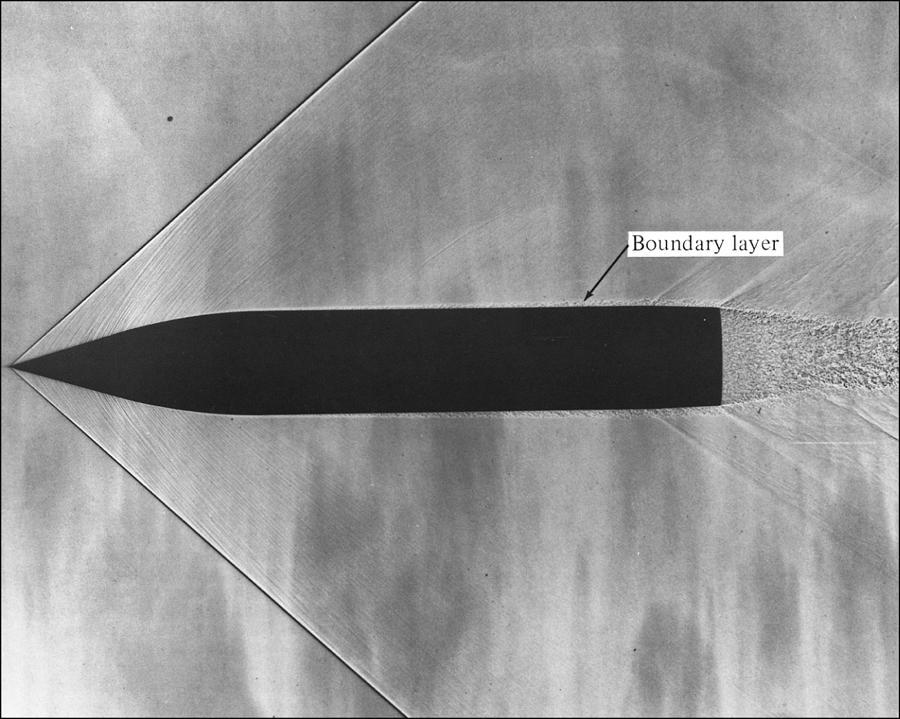
\includegraphics[width=0.9\textwidth]{Motivation/boundary_layer.png}\\
% Boundary layer
% \end{figure}
% \end{column}
% \end{columns}
% \end{frame}  


% ------------------------------------------------------------
\begin{frame}[t]
\frametitle{Motivation}
\framesubtitle{Initial Mesh Design is Expensive and Time-Consuming}
Stability requirements of numerical methods dictate that mesh must anticipate solution.
\begin{columns}[t]
\begin{column}[c]{0.4\textwidth}
\begin{itemize}
  \item Surface mesh must accurately represent geometry
  \item Volume mesh needs sufficient resolution for asymptotic regime
  % Before we accurately know the flow features
  \item Boundary layer meshes must respect $y^+$ guidelines
  \item Engineers often forced to work by trial and error
  \item Bad in the context of HPC
\end{itemize}
\end{column}
\begin{column}[c]{0.6\textwidth}
\vspace{2ex}
\begin{figure}[t]
\centering
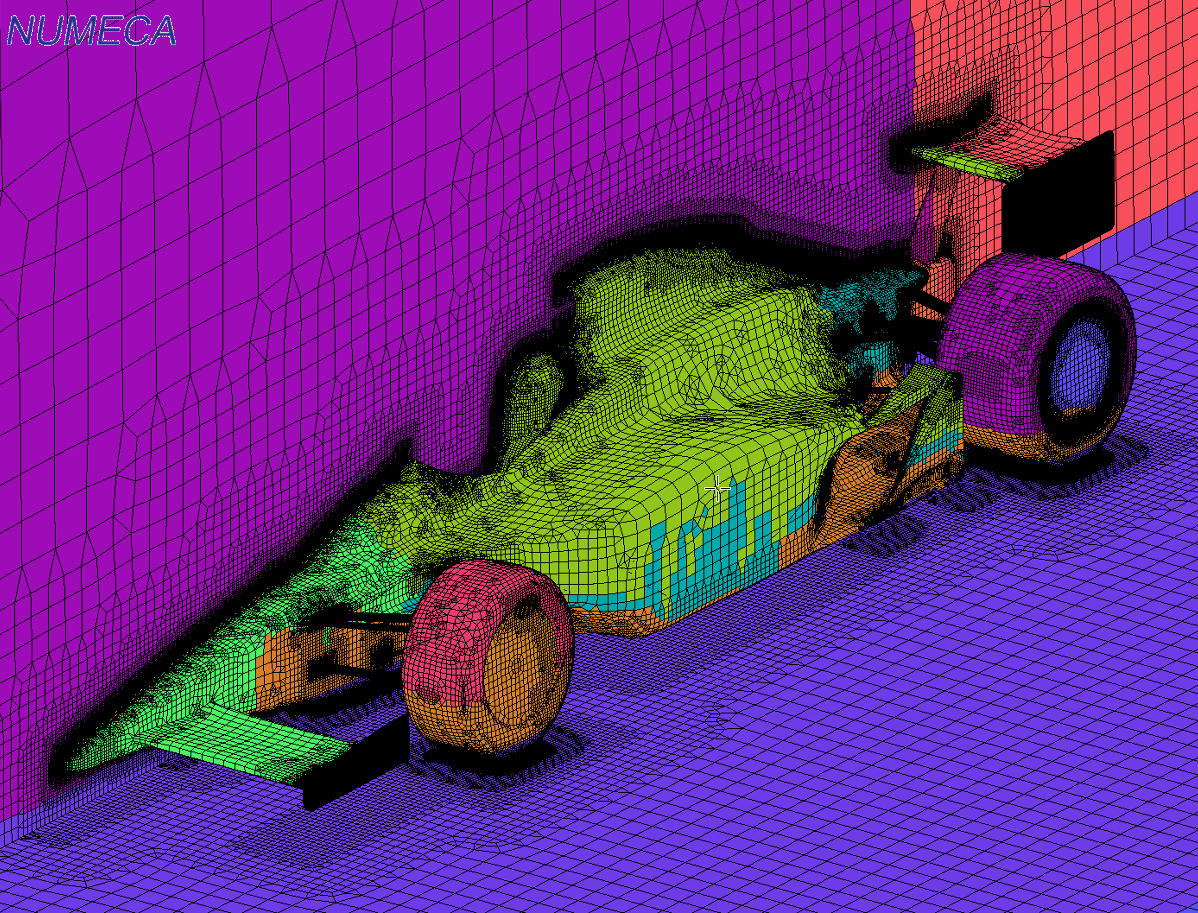
\includegraphics[width=1.0\textwidth]{Motivation/NumecaRaceCar.png}
\\\small{Formula 1 Mesh by Numeca}\\
\end{figure}
\end{column}
\end{columns}
\end{frame}


% ------------------------------------------------------------
\begin{frame}[t]
\frametitle{DPG on Coarse Meshes}
\framesubtitle{Adaptive Solve of the Carter Plate Problem\footfullcite{JesseDissertation} $Re=1000$}
\begin{columns}
\begin{column}{0.49\textwidth}
\begin{figure}
\centering

\includegraphics[width=1.0\textwidth]{Motivation/PlateMovie/T0.png}\\
\vspace{-1ex}
{\scriptsize Temperature on Initial Mesh}\\
\vspace{1ex}
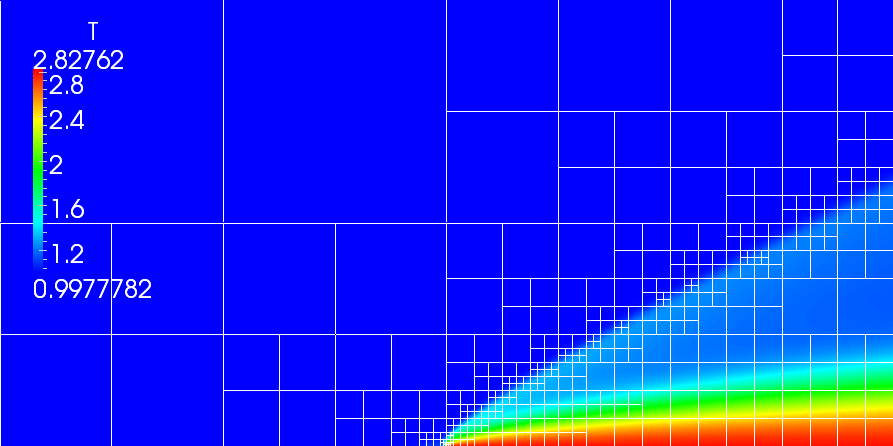
\includegraphics[width=1.0\textwidth]{Motivation/PlateMovie/T8.png}
\vspace{-1ex}
{\scriptsize Temperature after 8 Refinements}
\vspace{1ex}

\end{figure}
\end{column}
\begin{column}{0.49\textwidth}
\begin{figure}
\centering
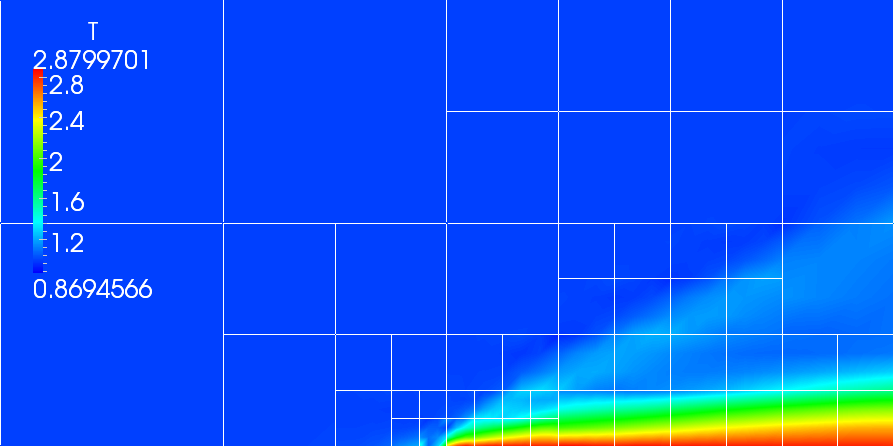
\includegraphics[width=1.0\textwidth]{Motivation/PlateMovie/T4.png}\\
\vspace{-1ex}
{\scriptsize Temperature after 4 Refinements}\\
\vspace{1ex}
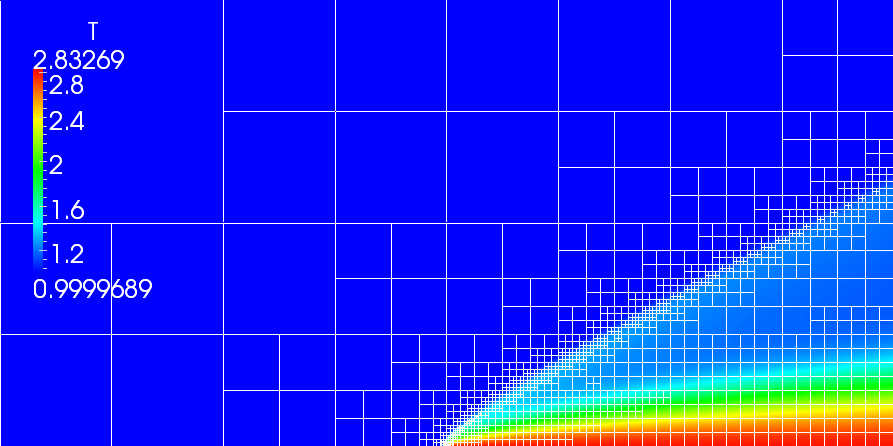
\includegraphics[width=1.0\textwidth]{Motivation/PlateMovie/T11.png}
\vspace{-1ex}
{\scriptsize Temperature after 11 Refinements}
\vspace{1ex}
\end{figure}
\end{column}
\end{columns}
\end{frame}



%   /$$$$$$$  /$$$$$$$   /$$$$$$         /$$$$$$                                            /$$                        
%  | $$__  $$| $$__  $$ /$$__  $$       /$$__  $$                                          |__/                        
%  | $$  \ $$| $$  \ $$| $$  \__/      | $$  \ $$ /$$    /$$  /$$$$$$   /$$$$$$  /$$    /$$ /$$  /$$$$$$  /$$  /$$  /$$
%  | $$  | $$| $$$$$$$/| $$ /$$$$      | $$  | $$|  $$  /$$/ /$$__  $$ /$$__  $$|  $$  /$$/| $$ /$$__  $$| $$ | $$ | $$
%  | $$  | $$| $$____/ | $$|_  $$      | $$  | $$ \  $$/$$/ | $$$$$$$$| $$  \__/ \  $$/$$/ | $$| $$$$$$$$| $$ | $$ | $$
%  | $$  | $$| $$      | $$  \ $$      | $$  | $$  \  $$$/  | $$_____/| $$        \  $$$/  | $$| $$_____/| $$ | $$ | $$
%  | $$$$$$$/| $$      |  $$$$$$/      |  $$$$$$/   \  $/   |  $$$$$$$| $$         \  $/   | $$|  $$$$$$$|  $$$$$/$$$$/
%  |_______/ |__/       \______/        \______/     \_/     \_______/|__/          \_/    |__/ \_______/ \_____/\___/ 
%                                                                                                                      
%                                                                                                                      
% 
\section{DPG Overview}
% ------------------------------------------------------------
\begin{frame}[t]
\frametitle{Overview of DPG}
\framesubtitle{DPG is a Minimum Residual Method}
Find $u\in U$ such that
\[
b(u,v)=l(v)\quad\forall v\in V
\]
with operator $B:U\rightarrow V'$ defined by $b(u,v)=\LRa{Bu,v}_{V'\times V}$.

This gives the operator equation 
\[
Bu=l\quad\in V'\,.
\]
We wish to minimize the residual $Bu-l\in V'$:
\[
u_h=\argmin_{w_h\in U_h}\frac{1}{2}\norm{Bu-l}^2_{V'}\,.
\]
Dual norms are not computationally tractable. 
Inverse Riesz map moves the residual to a more accessible space:
\[
u_h=\argmin_{w_h\in U_h}\frac{1}{2}\norm{R_V^{-1}(Bu-l)}^2_{V}\,.
\]
\end{frame}


% ------------------------------------------------------------
\begin{frame}[t]
\frametitle{Overview of DPG}
\framesubtitle{DPG is a Minimum Residual Method}
% \framesubtitle{Optimal Petrov-Galerkin Methods}
Taking the G\^ateaux derivative to be zero in all directions $\delta u \in
U_h$ gives,
\[
\left(R_V^{-1}(Bu_h-l),R_V^{-1}B\delta u\right)_V = 0, \quad \forall \delta u \in U,
\]
which by definition of the Riesz map is equivalent to 
\begin{equation*}
\LRa{Bu_h-l,R_V^{-1}B\delta u_h}=0\quad\forall\delta u_h\in U_h\,,
\end{equation*}
with optimal test functions $v_{\delta u_h}\coloneqq R_V^{-1}B\delta u_h$ for each trial function $\delta u_h$.
\begin{block}{Resulting Petrov-Galerkin System}
This gives a simple bilinear form
\begin{equation*}
b(u_h,v_{\delta u_h})=l(v_{\delta u_h}),
\end{equation*}
with $v_{\delta u_h}\in V$ that solves the auxiliary problem
\begin{equation*}
\LRp{v_{\delta u_h},\delta v}_V=\LRa{R_Vv_{\delta u_h},\delta v}
=\LRa{B\delta u_h,\delta v}=b(\delta u_h,\delta v)\quad\forall\delta v\in V.
\end{equation*}
\end{block}
\end{frame}


% ------------------------------------------------------------
\begin{frame}[t]
\frametitle{Overview of DPG}
\framesubtitle{DPG is the Most Stable Petrov-Galerkin Method}
Babu\v{s}ka's theorem guarantees that \emph{discrete stability and approximability imply convergence}.
If bilinear form $b(u,v)$, with $M:=\norm{b}$ satisfies the discrete inf-sup condition 
with constant $\gamma_h$,
\[
\sup_{v_h\in V_h}\frac{|b(u,v)|}{\norm{v_h}_V}\geq\gamma_h\norm{u_h}_U\,,
\]
then the Galerkin error satisfies the bound
\[
\norm{u_h-u}_U\leq\frac{M}{\gamma_h}\inf_{w_h\in U_h}\norm{w_h-u}_U\,.
\]
Optimal test function realize the supremum guaranteeing that $\gamma_h\geq\gamma$.\\
\begin{block}{Energy Norm}
If we use the energy norm, $\norm{u}_E:=\norm{Bu}_{V'}$ in the error estimate, then $M=\gamma=1$.
Babu\v{s}ka's theorem
implies that the minimum residual method is the most stable Petrov-Galerkin method (assuming exact optimal test functions).
\end{block}
\end{frame}


% ------------------------------------------------------------
\begin{frame}[t]
\frametitle{Overview of DPG\footfullcite{DPGOverview2}}
\framesubtitle{Other Features}
\begin{block}{Discontinuous Petrov-Galerkin}
\begin{itemize}
  \item Continuous test space produces global solve for optimal test functions
  \item Discontinuous test space results in an embarrassingly parallel solve
\end{itemize}
\end{block}
\begin{block}{Hermitian Positive Definite Stiffness Matrix}
Property of all minimum residual methods
\[
b(u_h,v_{\delta u_h})=\LRp{v_{u_h},v_{\delta u_h}}_V=\overline{\LRp{v_{\delta u_h},v_{u_h}}_V}=\overline{b(\delta u_h,v_{u_h})}
\]
\end{block}
\begin{block}{Error Representation Function}
Energy norm of Galerkin error (residual) can be computed without exact solution
\[
\norm{u_h-u}_E=\norm{B(u_h-u)}_{V'}=\norm{Bu_h-l}_{V'}=\norm{R_V^{-1}(Bu_h-l)}_V
\]
\end{block}
\end{frame}


% ------------------------------------------------------------
\begin{frame}[t]
\frametitle{Overview of DPG}
\framesubtitle{High Performance Computing}
\begin{columns}[c]
\begin{column}{.5\textwidth}
Eliminates human intervention
\medskip

\begin{itemize}
  \item Stability
  \item Robustness
  \item Adaptivity
  \item Automaticity
  \item Compute intensive
  \item Embarrassingly parallel local solves
  \item Factorization recyclable
  \item Low communication
  \item SPD stiffness matrix
  \item Multiphysics
\end{itemize}

% Issues to be solved
% \begin{itemize}
%   \item Iterative solvers
% \end{itemize}
\end{column}
\begin{column}{.5\textwidth}
\vspace{-3ex}
\begin{figure}[t]
\centering
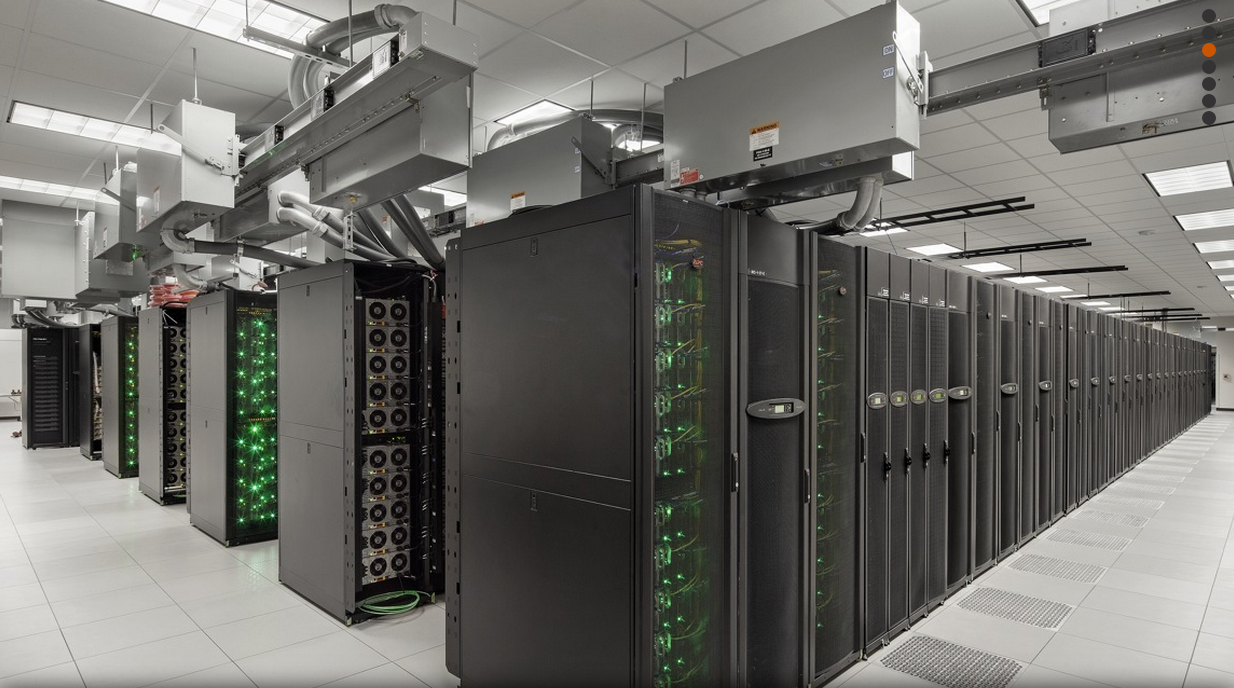
\includegraphics[width=0.9\textwidth]{Motivation/Stampede.png}
\\\small{Stampede Supercomputer at TACC}\\
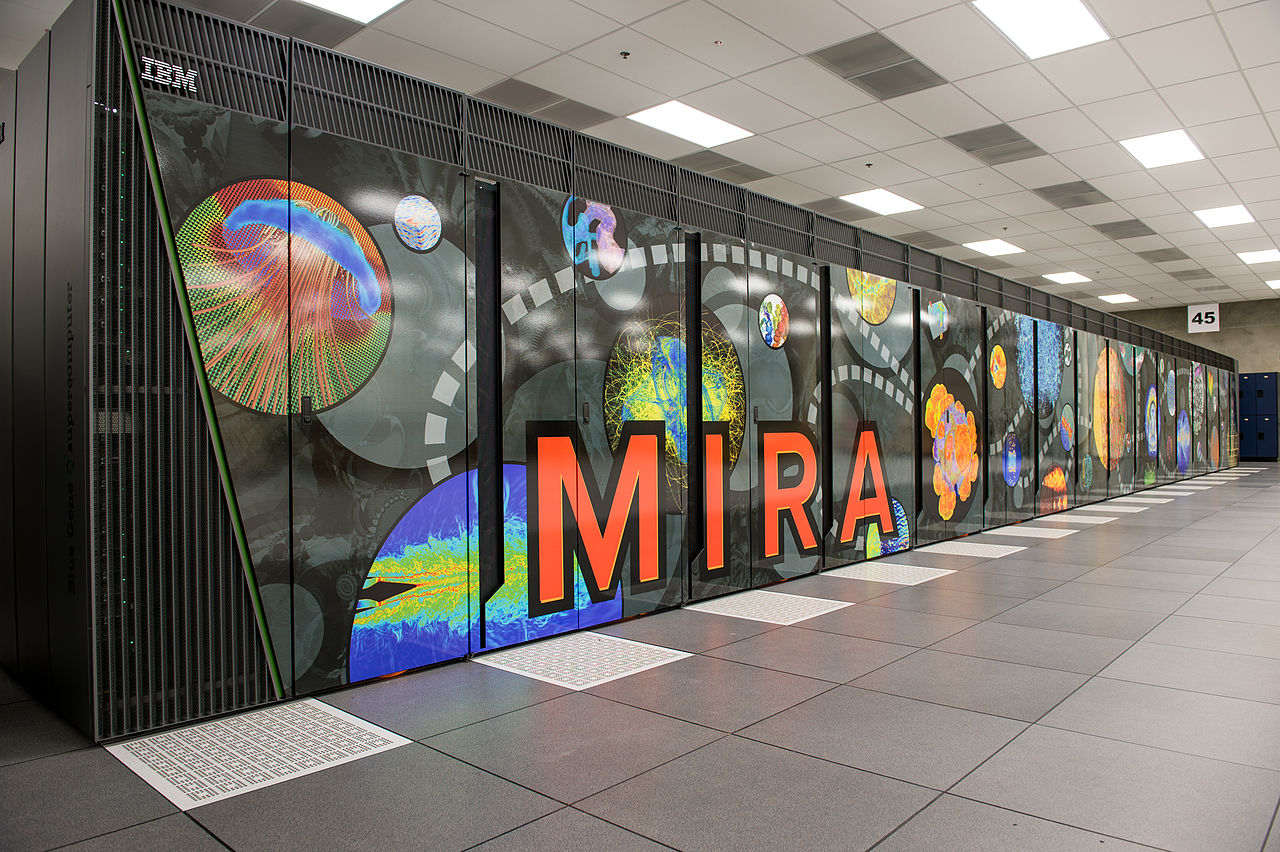
\includegraphics[width=0.9\textwidth]{Motivation/Mira.png}
\\\small{Mira Supercomputer at Argonne}\\
\end{figure}
\end{column}
\end{columns}

\end{frame}


% ------------------------------------------------------------
% \begin{frame}[t]
% \frametitle{Motivation}
% \framesubtitle{DPG for Massively Parallel CFD}  %% needed for proper positioning of the logo ...
% Pre-asymptotic stability and automatic adaptivity make a powerful synthesis.
% \begin{itemize}
%   \item Initial mesh design is a time consuming and expensive part of CFD.
%   \item Pre-asymptotic stability allows a DPG simulation to begin on the coarsest possible mesh.
%   \item Many methods become unstable in the pre-asymptotic regime.
%   \item Human intervention to correct a failed massively parallel simulation can be very costly.
%   \item Error indicator function indicates targets most important areas for refinement.
%   \item Provably robust for singularly perturbed problems.
% \end{itemize}

% \vspace{2ex}
% Space-time DPG extends these benefits to transient problems.
% \begin{itemize}
%   \item Localizes temporal adaptivity similar to spatial adaptivity.
% \end{itemize}
% \end{frame}



%    /$$$$$$                                                  /$$$$$$$$ /$$                        
%   /$$__  $$                                                |__  $$__/|__/                        
%  | $$  \__/  /$$$$$$   /$$$$$$   /$$$$$$$  /$$$$$$            | $$    /$$ /$$$$$$/$$$$   /$$$$$$ 
%  |  $$$$$$  /$$__  $$ |____  $$ /$$_____/ /$$__  $$ /$$$$$$   | $$   | $$| $$_  $$_  $$ /$$__  $$
%   \____  $$| $$  \ $$  /$$$$$$$| $$      | $$$$$$$$|______/   | $$   | $$| $$ \ $$ \ $$| $$$$$$$$
%   /$$  \ $$| $$  | $$ /$$__  $$| $$      | $$_____/           | $$   | $$| $$ | $$ | $$| $$_____/
%  |  $$$$$$/| $$$$$$$/|  $$$$$$$|  $$$$$$$|  $$$$$$$           | $$   | $$| $$ | $$ | $$|  $$$$$$$
%   \______/ | $$____/  \_______/ \_______/ \_______/           |__/   |__/|__/ |__/ |__/ \_______/
%            | $$                                                                                  
%            | $$                                                                                  
%            |__/  
\section{Space-Time DPG}


% ------------------------------------------------------------
\begin{frame}[t]
\frametitle{Space-Time DPG}
\framesubtitle{Motivation}
Extends the capabilities of a DPG solver
\begin{itemize}
  \item Preserves stability and robustness of DPG method
  \item Unified treatment of space and time
  \item Local space-time adaptivity (local time stepping)
  \begin{itemize}
    \item Small solution features require small time step
    \item Global time step not limited to smallest element
  \end{itemize}
  \item Natural framework for moving meshes
\end{itemize}
\bigskip

More computationally difficult
\begin{itemize}
  \item Solve requires $d+1$ dimensions
  \item Mesh structure more difficult
  \item Need to differentiate between spatial and temporal boundaries
  \item Larger global solves than finite difference time stepping
\end{itemize}
\end{frame}



%   /$$   /$$                       /$$    
%  | $$  | $$                      | $$    
%  | $$  | $$  /$$$$$$   /$$$$$$  /$$$$$$  
%  | $$$$$$$$ /$$__  $$ |____  $$|_  $$_/  
%  | $$__  $$| $$$$$$$$  /$$$$$$$  | $$    
%  | $$  | $$| $$_____/ /$$__  $$  | $$ /$$
%  | $$  | $$|  $$$$$$$|  $$$$$$$  |  $$$$/
%  |__/  |__/ \_______/ \_______/   \___/  
%                                          
%                                          
%  
% ------------------------------------------------------------
\begin{frame}[t]
\frametitle{Heat Equation}
\framesubtitle{Simplest Nontrivial Space-Time Problem}  %% needed for proper positioning of the logo ...

Equation is parabolic in space-time.
\begin{equation*}
  \frac{\partial u}{\partial t}-\epsilon\Delta u=f
\end{equation*}

This is really just a composite of Fourier's law and conservation of energy.
\begin{equation*}
\begin{aligned}
\bfsigma-\epsilon\Grad u&=0\\
\frac{\partial u}{\partial t}-\Div\bfsigma&=f
\end{aligned}
\end{equation*}

We can rewrite this in terms of a space-time divergence.
\begin{equation*}
\begin{aligned}
\frac{1}{\epsilon}\bfsigma-\Grad u&=0\\
\Divxt\vecttwo{-\bfsigma}{u}&=f
\end{aligned}
\end{equation*}
\end{frame}

% ------------------------------------------------------------
\begin{frame}[t]
\frametitle{Heat Equation}
\framesubtitle{DPG Formulation}  %% needed for proper positioning of the logo ...
% \vspace{-2ex}
Multiply by test function and integrate by parts over space-time element K.
\begin{equation*}
\begin{aligned}
\LRp{\frac{1}{\epsilon}\bfsigma,\bftau}+\LRp{u,\Div\bftau}-\LRa{\hat u,\bftau\cdot\bfn_x}&=0\\
-\LRp{\vecttwo{-\bfsigma}{u},\Gradxt v}+\LRa{\hat t,v}&=f
\end{aligned}
\end{equation*}
\begin{columns}[t] % contents are top vertically aligned
\begin{column}[T]{0.4\textwidth} % each column can also be its own environment
where
\begin{align*}
\hat u&:=\trace(u)\\
\hat t&:=\trace(-\bfsigma)\cdot\bfn_x+\trace(u)\cdot n_t
\end{align*}
\vspace{-4ex}
\begin{itemize}
  \item Trace $\hat u$ defined on spatial boundaries
  \item Flux $\hat t$ defined on all boundaries
\end{itemize}
\end{column}
\begin{column}[T]{0.6\textwidth} % alternative top-align that's better for graphics
\vspace{-2ex}
\begin{block}{Support of Trace Variables}
\begin{tikzpicture}[line cap=round,line join=round,>=triangle 45,x=2.0cm,y=2.0cm, scale=0.6, every node/.style={scale=0.6}]
\clip(-0.7,-0.6) rectangle (5.27,2.09);
\draw (0,2)-- (0,0);
\draw (0,0)-- (1,0);
\draw (1,0)-- (4,0);
\draw (4,0)-- (5,0);
\draw (5,0)-- (5,2);
\draw (5,2)-- (3,2);
\draw (3,2)-- (2,2);
\draw (2,2)-- (0,2);
\draw (1,0)-- (1.5,1);
\draw (1.5,1)-- (2,2);
\draw (1.5,1)-- (3.5,1);
\draw (3,2)-- (3.5,1);
\draw (3.5,1)-- (4,0);
\draw (-0.21,0.9) node[anchor=south west] {$\hat u$};
\draw (4.82,0.9) node[anchor=south west] {$\hat u$};
\draw (3.5,0.45) node[anchor=south west] {$\hat u$};
\draw (1.0,0.45) node[anchor=south west] {$\hat u$};
\draw (1.5,1.4) node[anchor=south west] {$\hat u$};
\draw (3.0,1.4) node[anchor=south west] {$\hat u$};
\draw (0.05,0.9) node[anchor=south west] {$\hat t$};
\draw (1.40,0.45) node[anchor=south west] {$\hat t$};
\draw (3.79,0.45) node[anchor=south west] {$\hat t$};
\draw (2.47,1.0) node[anchor=south west] {$\hat t$};
\draw (3.33,1.4) node[anchor=south west] {$\hat t$};
\draw (1.89,1.4) node[anchor=south west] {$\hat t$};
\draw (5.07,0.9) node[anchor=south west] {$\hat t$};
\draw (4.44,0.0) node[anchor=south west] {$\hat t$};
\draw (2.46,0.0) node[anchor=south west] {$\hat t$};
\draw (0.45,0.0) node[anchor=south west] {$\hat t$};
\draw (2.44,1.7) node[anchor=south west] {$\hat t$};
\draw (0.76,1.7) node[anchor=south west] {$\hat t$};
\draw (4.21,1.7) node[anchor=south west] {$\hat t$};
\draw [->] (-0.5,-0.5) -- (-0.5,0);
\draw [->] (-0.5,-0.5) -- (0,-0.5);
\draw (-0.54,0.29) node[anchor=north west] {$t$};
\draw (0.07,-0.35) node[anchor=north west] {$x$};
\end{tikzpicture}
\end{block}
\end{column}
\end{columns}
\end{frame}

% ------------------------------------------------------------
\begin{frame}[t]
\frametitle{Heat equation}
\framesubtitle{Pulsed Source Problem}  %% needed for proper positioning of the logo ...
\vspace{-1ex}
\begin{columns}[t] % contents are top vertically aligned
\begin{column}[c]{0.3\textwidth} % each column can also be its own environment
% \vspace{3ex}
\begin{itemize}
  \item Initial condition $u=0$.
  \item Apply unit source $x\in[3/8,5/8]$,\\$t\in[1/4,1/2]$.
  \item Should not violate causality
  \item Space-time adaptivity picks up areas of rapid change.
\end{itemize}
\end{column}
\begin{column}[c]{0.7\textwidth} % each column can also be its own environment
\begin{figure}[ht]
\centering
\begin{subfigure}[t]{0.45\textwidth}
\centering
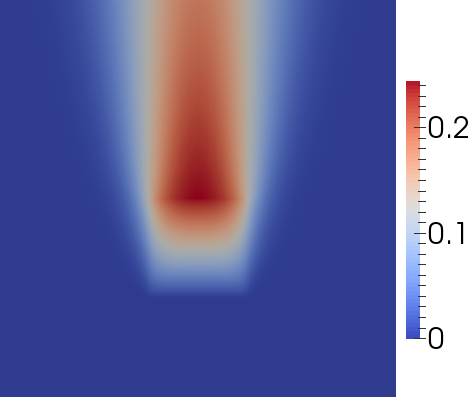
\includegraphics[height=0.8\textwidth]{SpaceTimeHeat/PulseSource/u.png}
\\$u$\\\vspace{1ex}
\end{subfigure}
\begin{subfigure}[t]{0.45\textwidth}
\centering
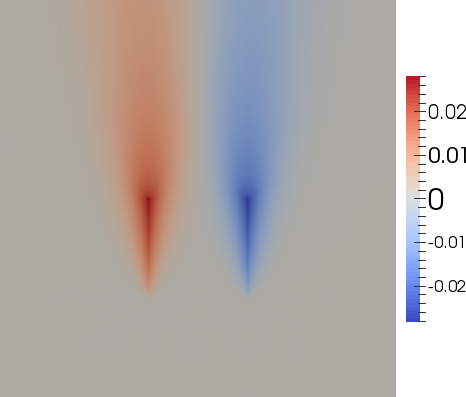
\includegraphics[height=0.8\textwidth]{SpaceTimeHeat/PulseSource/sigma.png}
\\$\sigma$\\\vspace{1ex}
\end{subfigure}
\begin{subfigure}[t]{0.45\textwidth}
\centering
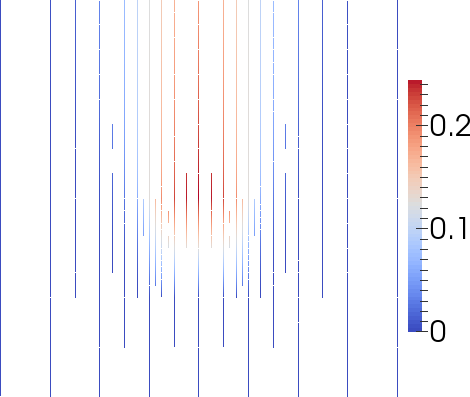
\includegraphics[height=0.8\textwidth]{SpaceTimeHeat/PulseSource/uhat.png}
\\$\hat u$
\end{subfigure}
\begin{subfigure}[t]{0.45\textwidth}
\centering
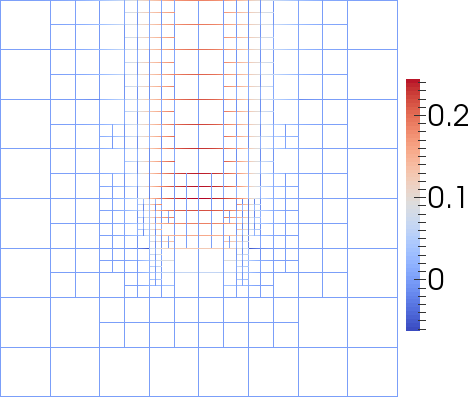
\includegraphics[height=0.8\textwidth]{SpaceTimeHeat/PulseSource/fhat.png}
\\$\hat t$
\end{subfigure}
% \caption{Pulsed space-time heat problem after 4 refinements}
\end{figure}
\end{column}
\end{columns}
\end{frame}

%    /$$$$$$                                                                            /$$ /$$       /$$          
%   /$$__  $$                                                                          |__/| $$      | $$          
%  | $$  \__/  /$$$$$$  /$$$$$$/$$$$   /$$$$$$   /$$$$$$   /$$$$$$   /$$$$$$$  /$$$$$$$ /$$| $$$$$$$ | $$  /$$$$$$ 
%  | $$       /$$__  $$| $$_  $$_  $$ /$$__  $$ /$$__  $$ /$$__  $$ /$$_____/ /$$_____/| $$| $$__  $$| $$ /$$__  $$
%  | $$      | $$  \ $$| $$ \ $$ \ $$| $$  \ $$| $$  \__/| $$$$$$$$|  $$$$$$ |  $$$$$$ | $$| $$  \ $$| $$| $$$$$$$$
%  | $$    $$| $$  | $$| $$ | $$ | $$| $$  | $$| $$      | $$_____/ \____  $$ \____  $$| $$| $$  | $$| $$| $$_____/
%  |  $$$$$$/|  $$$$$$/| $$ | $$ | $$| $$$$$$$/| $$      |  $$$$$$$ /$$$$$$$/ /$$$$$$$/| $$| $$$$$$$/| $$|  $$$$$$$
%   \______/  \______/ |__/ |__/ |__/| $$____/ |__/       \_______/|_______/ |_______/ |__/|_______/ |__/ \_______/
%                                    | $$                                                                          
%                                    | $$                                                                          
%                                    |__/    

% ------------------------------------------------------------
\begin{frame}[t]
\frametitle{Compressible Navier-Stokes}
\framesubtitle{Strong Form}  %% needed for proper positioning of the logo ...
The compressible Navier-Stokes equations are
\begin{align*}
\frac{\partial}{\partial t}\svectthree{\rho}{\rho\bfu}{\rho e_0}
+\Div\svectthree{\rho\bfu}{\rho\bfu\otimes\bfu+p\bfI-\mathbb{D}}{\rho\bfu e_0+\bfu p+\bfq-\bfu\cdot\mathbb{D}}
%TODO: Possible error above. cfd-online seems to have T^T
=\svectthree{f_c}{\bff_m}{f_e}\,,
\end{align*}
where
\begin{equation*}
  \mathbb{D}=2\mu\bfS^*=2\mu\LRs{\frac{1}{2}\LRp{\Grad\bfu+\LRp{\Grad\bfu}^T}-\frac{1}{3}\Div\bfu\bfI}\,,
\end{equation*}
\begin{equation*}
  \bfq=-C_p\frac{\mu}{Pr}\Grad T\,,
\end{equation*}
and (assuming an ideal gas EOS)
\[
p=\rho R T\,.
\]
\end{frame}

% ------------------------------------------------------------
\begin{frame}[t]
\frametitle{Compressible Navier-Stokes}
\framesubtitle{First Order Space-Time Form}  %% needed for proper positioning of the logo ...
Writing this in space-time in terms of $\rho$, $\bfu$, $T$, $\mathbb{D}$, and $\bfq$:
\begin{align*}
  \mathbb{D}-\mu\LRp{\Grad\bfu+\LRp{\Grad\bfu}^T}+\frac{2\mu}{3}\Div\bfu\bfI&=0\\
  \bfq+C_p\frac{\mu}{Pr}\Grad T&=0\\
  \Divxt\vecttwo{\rho\bfu}{\rho}&=f_c\\
  \Divxt\vecttwo{\rho\bfu\otimes\bfu+\rho RT\bfI-\mathbb{D}}{\rho\bfu}&=\bff_m\\
  \Divxt\vecttwo{\rho\bfu\LRp{C_v T+\frac{1}{2}\bfu\cdot\bfu}+\bfu\rho RT+\bfq-\bfu\cdot\mathbb{D}}{\rho\LRp{C_v T+\frac{1}{2}\bfu\cdot\bfu}}&=f_e\,.
\end{align*}
\end{frame}


% ------------------------------------------------------------
\begin{frame}[t]
\frametitle{Compressible Navier-Stokes}
\framesubtitle{DPG Formulation}  %% needed for proper positioning of the logo ...
Multiplying by test functions and integrating by parts:
% \scalebox{0.9}{
{
\small
\begin{align*}
  \LRp{\mathbb{D},\mathbb{S}}+\LRp{2\mu\bfu,\Div\mathbb{S}}-\LRp{\frac{2\mu}{3}\bfu,\Grad\trace{\mathbb{S}}}
  -\LRa{2\mu\hat\bfu,\mathbb{S}\bfn_x}+\LRa{\frac{2\mu}{3}\hat\bfu,\mathbb{S}\bfn_x}&=0\\
  \LRp{\bfq,\bftau}-\LRp{C_p\frac{\mu}{Pr}T,\Div\bftau}+\LRa{C_p\frac{\mu}{Pr}\hat T,\tau_n}&=0\\
  -\LRp{\vecttwo{\rho\bfu}{\rho},\Gradxt v_c}+\LRa{\hat t_c,v_c}&=\LRp{f_c,v_c}\\
  -\LRp{\vecttwo{\rho\bfu\otimes\bfu+\rho RT\bfI-\mathbb{D}}{\rho\bfu},\Gradxt\bfv_m}+\LRa{\hat\bft_m,\bfv_m}&=\LRp{\bff_m,\bfv_m}\\
  -\LRp{\vecttwo{\rho\bfu\LRp{C_v T+\frac{1}{2}\bfu\cdot\bfu}+\bfu\rho RT+\bfq-\bfu\cdot\mathbb{D}}{\rho\LRp{C_v T+\frac{1}{2}\bfu\cdot\bfu}},\Gradxt v_e}
  +\LRa{\hat t_e,v_e}&=\LRp{f_e,v_e}\,,
\end{align*}
}
% }
where $\hat u$ and $\hat T$ are spatial traces and $\hat t_c$, $\hat\bft_m$, and $\hat t_e$ are fluxes.
\end{frame}


% ------------------------------------------------------------
\begin{frame}[t]
\frametitle{Compressible Navier-Stokes}
\framesubtitle{Flux and Trace Variables}  %% needed for proper positioning of the logo ...
Spatial traces and fluxes are defined as follows:
\begin{equation*}
\begin{aligned}
\hat\bfu&=\trace(\bfu)\\
\hat T&=\trace(T)\\
\hat t_c&=\trace\LRp{\rho\bfu}\cdot\bfn_x
+\trace\LRp{\rho}n_t\\
\hat\bft_m&=\trace\LRp{\rho\bfu\otimes\bfu+\rho RT\bfI-\mathbb{D}}\cdot\bfn_x
+\trace\LRp{\rho\bfu} n_t\\
\hat t_e&=\trace\LRp{\rho\bfu\LRp{C_v T+\frac{1}{2}\bfu\cdot\bfu}+\bfu\rho RT+\bfq-\bfu\cdot\mathbb{D}}\cdot\bfn_x\\
&\quad+\trace\LRp{\rho\LRp{C_v T+\frac{1}{2}\bfu\cdot\bfu}}n_t\,.
\end{aligned}
\end{equation*}
\begin{block}{Linearization}
Fluxes, traces, and $\bfq$ are linear in the above bilinear form, but we need to linearize in $\rho$, $\bfu$, $T$, and $\mathbb{D}$ 
(Jacobian and residual not shown here).
\end{block}
\end{frame}


%TODO: Fix test norm
% ------------------------------------------------------------
\begin{frame}[t]
\frametitle{Compressible Navier-Stokes}
\framesubtitle{Test Norm}  %% needed for proper positioning of the logo ...
\vspace{-3ex}
{
\small
\begin{align*}
&\norm{\Grad\bfv_m+\Grad v_e\otimes\tilde\bfu}^2+\norm{\Grad v_e}^2\\
+&\left\|
-\tilde\bfu\cdot\Grad v_c-\frac{\partial v_c}{\partial t}-\tilde\bfu\otimes\tilde\bfu:\Grad\bfv_m
-R\tilde T\Div\bfv_m-\tilde\bfu\cdot\frac{\partial\bfv_m}{\partial t}\right.\\
&\left.-C_v\tilde T\tilde\bfu\cdot\Grad v_e-\frac{1}{2}\tilde\bfu\cdot\tilde\bfu\tilde\bfu\cdot\Grad v_e
-R\tilde T\tilde\bfu\Grad v_e
-C_v\tilde T\frac{\partial v_e}{\partial t}-\frac{1}{2}\tilde\bfu\cdot\tilde\bfu\frac{\partial v_e}{\partial t}
\right\|^2\\
+&\left\|
-\tilde\rho\Grad v_c
-\tilde\rho\tilde\bfu\cdot\Grad\bfv_m-\tilde\rho\Grad\bfv_m\cdot\tilde\bfu
-\tilde\rho\frac{\partial\bfv_m}{\partial t}
-C_v\tilde\rho\tilde T\Grad v_e
-\frac{1}{2}\tilde\rho\tilde\bfu\cdot\tilde\bfu\Grad v_e
\right.\\
&\left.
-\frac{1}{2}\tilde\rho\tilde\bfu\cdot\Grad v_e\tilde\bfu
-\frac{1}{2}\tilde\rho\Grad v_e\cdot\tilde\bfu\tilde\bfu
-R\tilde\rho\tilde T\Grad v_e
+\tilde{\mathbb{D}}\cdot\Grad v_e
-\frac{1}{2}\tilde\rho\tilde\bfu\frac{\partial v_e}{\partial t}
-\frac{1}{2}\tilde\rho\tilde\bfu\frac{\partial v_e}{\partial t}
\right\|^2\\
+&\left\|
-R\tilde\rho\Div\bfv_m
-C_v\tilde\rho\tilde\bfu\Grad v_e
-R\tilde\rho\tilde\bfu\Grad v_e
-C_v\tilde\rho\frac{\partial v_e}{\partial t}
\right\|^2\\
+&\|\frac{1}{\mu}\mathbb{S}\|^2
+\norm{2\Div\mathbb{S}-\frac{2}{3}\Grad\trace{\mathbb{S}}}^2
+\|\frac{Pr}{C_p\mu}\bftau\|^2
+\norm{\Div\bftau}^2\\
+&\norm{v_c}^2+\norm{\bfv_m}^2+\norm{v_e}^2
\,.
\end{align*}
}
\end{frame}


%    /$$$$$$                  /$$                     
%   /$$__  $$                | $$                     
%  | $$  \__/  /$$$$$$   /$$$$$$$  /$$$$$$  /$$    /$$
%  |  $$$$$$  /$$__  $$ /$$__  $$ /$$__  $$|  $$  /$$/
%   \____  $$| $$$$$$$$| $$  | $$| $$  \ $$ \  $$/$$/ 
%   /$$  \ $$| $$_____/| $$  | $$| $$  | $$  \  $$$/  
%  |  $$$$$$/|  $$$$$$$|  $$$$$$$|  $$$$$$/   \  $/   
%   \______/  \_______/ \_______/ \______/     \_/    
%                                                     
%                                                     
% 
% ------------------------------------------------------------
\begin{frame}[t]
\frametitle{Compressible Navier-Stokes}
\framesubtitle{Sod Shock Tube with $\mu=10^{-5}$}  %% needed for proper positioning of the logo ...
\foreach \n in {1,...,15}
{
\only<\n>
{
\vspace{-2ex}
\begin{figure}[ht]
\centering

\begin{subfigure}[c]{0.45\textwidth}
\centering
\includegraphics[height=0.7\textwidth]{SpaceTimeCNS/Sod1e-5/den\n.pdf}
\end{subfigure}
\begin{subfigure}[c]{0.45\textwidth}
\centering
\includegraphics[height=0.7\textwidth]{SpaceTimeCNS/Sod1e-5/vel\n.pdf}
\end{subfigure}
\begin{subfigure}[c]{0.45\textwidth}
\centering
\includegraphics[height=0.7\textwidth]{SpaceTimeCNS/Sod1e-5/pres\n.pdf}
\end{subfigure}
\begin{subfigure}[c]{0.45\textwidth}
\centering
\includegraphics[width=1\textwidth]{SpaceTimeCNS/Sod1e-5/mesh\n.png}
\end{subfigure}
\end{figure}
}
}
\end{frame}


%   /$$   /$$           /$$      
%  | $$$ | $$          | $$      
%  | $$$$| $$  /$$$$$$ | $$$$$$$ 
%  | $$ $$ $$ /$$__  $$| $$__  $$
%  | $$  $$$$| $$  \ $$| $$  \ $$
%  | $$\  $$$| $$  | $$| $$  | $$
%  | $$ \  $$|  $$$$$$/| $$  | $$
%  |__/  \__/ \______/ |__/  |__/
%                                
%                                
% 
% ------------------------------------------------------------
% \begin{frame}[t]
% \frametitle{Compressible Navier-Stokes}
% \framesubtitle{Noh Implosion with $\mu=10^{-3}$}  %% needed for proper positioning of the logo ...
% Infinitely strong shock propagation.
% \foreach \n in {1,...,9}
% {
% \only<\n>
% {
% \vspace{4ex}
% \begin{columns}[t] % contents are top vertically aligned
% \begin{column}[T]{0.45\textwidth} % each column can also be its own environment
% \centering
% \includegraphics[height=1.0\textwidth]{SpaceTimeCNS/Noh1e-3/den\n.pdf}
% \end{column}
% \hspace{8ex}
% \begin{column}[T]{0.45\textwidth} % each column can also be its own environment
% \centering
% \vspace{2ex}
% \includegraphics[width=0.9\textwidth]{SpaceTimeCNS/Noh1e-3/mesh\n.png}
% \end{column}
% \end{columns}
% }
% }
% \end{frame}


\section{Conclusions and Future Work}
\begin{frame}[t]
\frametitle{Conclusions and Future Work}
\framesubtitle{~~}Conclusions
\begin{itemize}
  \item A problem in conservation form can be transformed to a space-time divergence.
  \item Fluxes change character from spatial to temporal boundaries.
  \item Traces are only defined on spatial boundaries.
\end{itemize}
\bigskip

Future Work
\begin{itemize}
  \item Proof of robustness for convection-diffusion.
  \item Analysis of robust test norms.
  \item Time slabs will reduce the simulation cost.
  \item Two and three dimensions for more realistic problems.
  \item Incompressible Navier-Stokes.
  \item Iterative solvers for parallel scalability.
\end{itemize}
\end{frame}


\begin{frame}[t]
\frametitle{Thank You!}
\framesubtitle{~~}
\vspace{-4ex}
\begin{figure}[ht]
\centering
\begin{subfigure}[c]{0.45\textwidth}
\centering
\animategraphics[autoplay,loop,width=0.99\textwidth]{1}{SpaceTimeCNS/Sod1e-5/den}{1}{15}
\end{subfigure}
\begin{subfigure}[c]{0.45\textwidth}
\centering
\animategraphics[autoplay,loop,width=0.99\textwidth]{1}{SpaceTimeCNS/Sod1e-5/vel}{1}{15}
\end{subfigure}
\begin{subfigure}[c]{0.45\textwidth}
\centering
\animategraphics[autoplay,loop,width=0.99\textwidth]{1}{SpaceTimeCNS/Sod1e-5/pres}{1}{15}
\end{subfigure}
\begin{subfigure}[c]{0.45\textwidth}
\centering
\animategraphics[autoplay,loop,width=0.99\textwidth]{1}{SpaceTimeCNS/Sod1e-5/mesh}{1}{15}
\end{subfigure}
\end{figure}
\end{frame}


% \begin{frame}[t]
% \frametitle{Bibliography}
% \framesubtitle{~~}  %% needed for proper positioning of the logo ...
% {\oldfootnotesize
% \printbibliography
% }
% \end{frame}

\end{document}
